
\documentclass[a4paper,12pt]{article}
\usepackage[margin=1in]{geometry}
\renewcommand{\tabcolsep}{1 mm}
\usepackage[T2A]{fontenc}			% кодировка
\usepackage[utf8]{inputenc}			% кодировка исходного текста
\usepackage[english,russian]{babel}	% локализация и переносы
\usepackage{graphicx}                % Математика
\usepackage{amsmath,amsfonts,amssymb,amsthm,mathtools} 
\usepackage{mathtext}
\usepackage[T2A]{fontenc}
\usepackage[utf8]{inputenc}

\usepackage{wasysym}

%Заговолок
\author{Бичина Марина 
группа Б04-005 1 курса ФЭФМ}
\title{Отчет по лабораторной работе №2.4.1


Определение теплоты испарения жидкости}
\date{02.03.2021}


\begin{document} % начало документа

\maketitle
\newpage

\section{Аннотация}

\paragraph{Цель работы:} 
\begin{enumerate}
\itemsep0em
\item Измерить давление насыщенного пара жидкости при разной температуре 
\item Вычислить по полученным денным теплоты испарения с помощью уравнения Клапейрона-Клаузиуса
\end{enumerate}
\paragraph{Оборудование:}
\begin{enumerate}
\itemsep0em
\item термостат
\item герметичный сосуд, заполненный исследуемой жидкостью
\item отсчетный микроскоп
\end{enumerate}
\section{Теоретическая часть}

\paragraph{} Испарением называется переход вещества из жидкого в газообразное состояние. Оно происходит на свободной поверхности жидкости. При испарении с поверхности вылетают молекулы, образуя над ней пар. Для выхода из жидкости молекулы должны преодолеть силы молекулярного сцепления. Кроме того, при испарении совершается работа против внешнего давления $P$, поскольку объем жидкости меньше объема пара. Не все молекулы жидкости способны совершить эту работу, а только те из них, которые обладают достаточной кинетической энергией. Поэтому переход части молекул в пар приводит к обеднению жидкости быстрыми молекулами, т. е. к ее охлаждению. Чтобы испарение проходило без изменения температуры, к жидкости нужно подводить тепло. Количество теплоты, необходимое для изотермического испарения одного моля жидкости при внешнем давлении, равном упругости ее насыщенных паров, называется \textit{молярной теплотой испарения (парообразования)}.


Измерение с помощью калориметра является весьма неточной из-за неконтролируемых потерь тепла, которые трудно сделать малыми. Поэтому в настоящей работе для определения теплоты испарения применен косвенный метод, основанный на формуле Клапейрона-Клаузиуса

\begin{equation}
\frac{dP}{dT}=\frac{L}{T(V_2-V_1)}
\end{equation}
Где $P$ — давление насыщенного пара жидкости при температуре $T$, $T$ — абсолютная температура жидкости и пара, $L$ — теплота испарения жидкости, $V_2$ — объем пара, $V_1$ — объем жидкости.

С помощью уравнения Ван-дер-Ваальса можно получить зависимость $P(T)$, с помощью которой определить искомую величину. 

\begin{equation*}
(P+\frac{a}{V^2})(V-b)=RT
\end{equation*}


В нашем приборе измерения производятся при давлениях ниже
атмосферного.В этом случае задача существенно упрощается. В таблице (1) для ряда жидкостей приведены: температура, при которой давление насыщенных паров равно атмосферному, величины $V_2$ и $V_1$, входящие в (1), а также константы $a$ и $b$ в уравнении Ван-дер-Ваальса.
\begin{center}
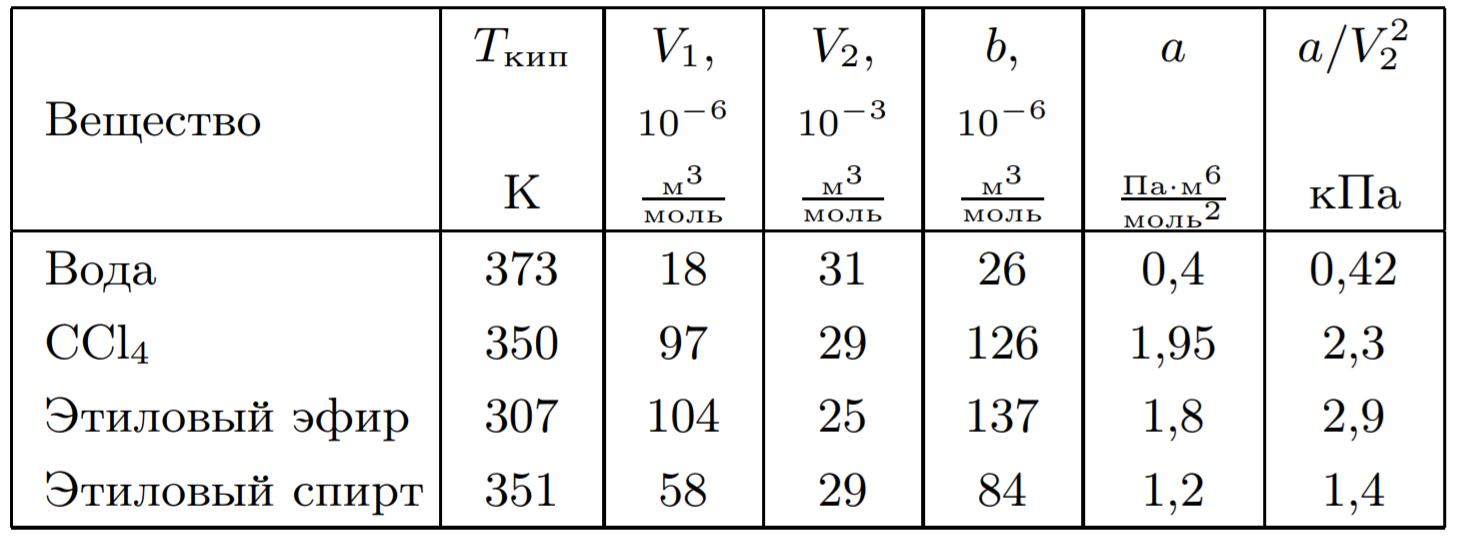
\includegraphics[width=0.7\linewidth]{tab.png}
\end{center}

 Откуда видно, что $\frac{V_1}{V_2} < 0.005$, a $\frac{a}{PV^2}<0.03$, ошибка метода измерений равна 4\%, тогда
 
 \begin{equation*}
PV=\nu RT
\end{equation*} \\
\begin{equation}
L=\frac{ RT^2}{P}\frac{dP}{dT} = - R\frac{d(lnP)}{d(\frac{1}{T})}
\end{equation}
(2) -- окончательная формула для вычисления теплоты испарения жидкости.
\subsection{Описание установки:}
\paragraph{Систематические погрешности:}
\begin{enumerate}
\itemsep0em
\item Термометр: 0,2 К
\item Штангенциркуль: 0,1 мм
\end{enumerate}

\begin{figure}[h]
\begin{center}
\begin{minipage}[h]{0.4\linewidth}
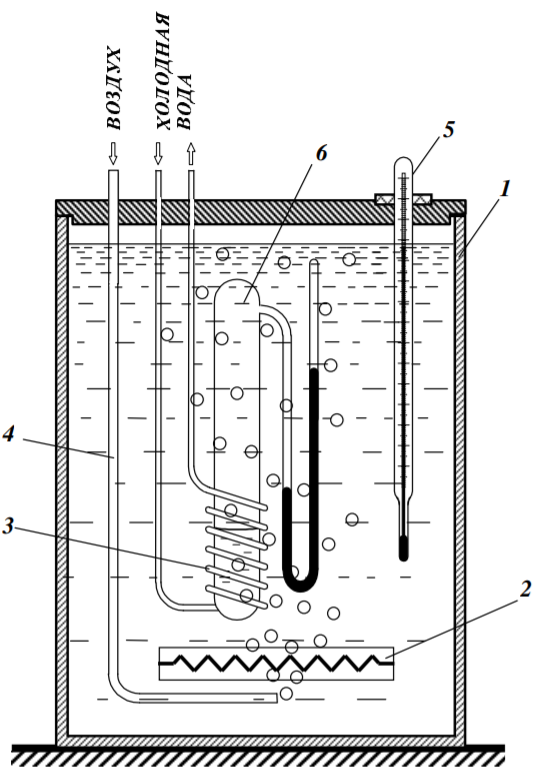
\includegraphics[width=0.65\linewidth]{ustanovka_1.png}
\caption{Схема установки для определения теплоты испарения}
\label{ris:ustanovka_1} 
\end{minipage}
\hfill
\begin{minipage}[h]{0.5\linewidth}
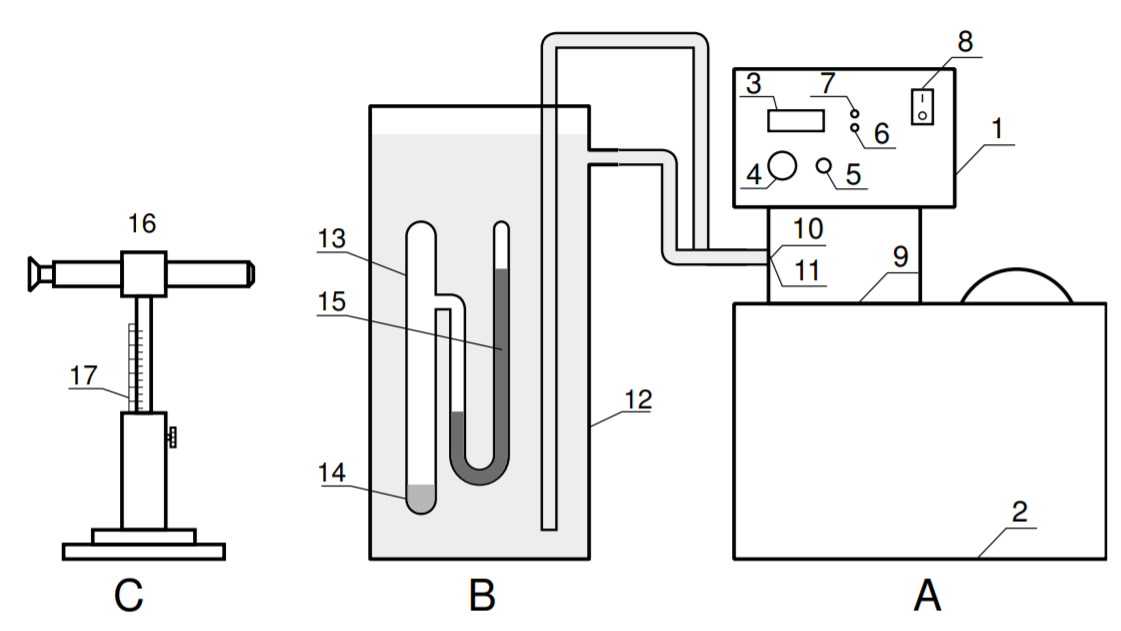
\includegraphics[width=1.3\linewidth]{ustanovka_2.png}
\caption{Схема установки для определения теплоты испарения}
\label{ris:ustanovka_2}
\end{minipage}
\end{center}
\end{figure}

\paragraph{На рисунке 1 изображены:} 
\begin{enumerate}
\itemsep0em
\item Резервуар, наполенный водой
\item Спираль, подогреваемая электрическим током
\item Змеевик, через который происходит охлаждение
\item Труба, через которую поступает воздух
\item Термометр
\item Прибор с исследуемой жидкостью
\end{enumerate}

\paragraph{}На рисунке 2 представлена другая версия установки, где:

A -- термостат, B -- экспериментальный прибор, C --  отсчетный микроскоп. 
Экспериментальный прибор В и отсчетный микроскоп С представляют собой:
\begin{enumerate}
\itemsep0em
\setcounter{enumi}{11}
\item Емкость, заполненную водой
\item Запаянный прибор 
\item Исследуемая жидкость 
\item Ртутный манометр
\item Отсчетный микроскоп
\item Шкала, по которой снимаются показания
\end{enumerate}

У нас была 1 установка
\subsection{Контрольные вопросы:}
\begin{enumerate}
\itemsep0em
\item В справочниках приводится теплота испарения, измеренная при давлении 760 мм рт. ст. Совпадает ли эта величина с измеренной нами на опыте? Какая из них больше? Оценить разницу между ними

	Полученные в ходе эксперимента данные получились больше табличных на 13\%:

  $L = 45200 \pm 600 \; \frac{\text{Дж}}{\text{моль}}$,  $L = 40680 \; \frac{\text{Дж}}{\text{моль}}$
\item Указать, исходя из теоретических соображений, в какую сторону должна меняться теплота испарения с увеличением температуры.

	Уменьшается, так как состояние жидкости приближается к критическому, в котором фазовый переход происходит без затрат энергии.

\end{enumerate}
\section{Ход работы:}
\begin{enumerate}
\itemsep0em
\item Измерим разность уровней в ртутном U-образном манометре с помощью микроскопа и температуру по термометру или индикаторному
табло. У нас это 
\begin{equation*}
\Delta h_0 = 18 \pm 0,1 \text{мм}
\end{equation*} 
\item Включим термостат. Поскольку мы работаем по схеме на  рис. 1, то подогреем воду в калориметре, пропуская ток через нагреватель. Через каждый градус измеряем давление и температуру.
Продолжаем повышать температуру в течение половины имеющегося у нас времени.
\item Проведем те же измерения при охлаждении жидкости.
Установим такой поток воды, чтобы охлаждение шло примерно тем же темпом, что и нагревание.
\\ 
\item Вычислим изменение разности уровней в манометре при нагревании и при охлаждении 
\item Посчитаем давление в мм рт. ст. $\Delta h = \Delta h_0 + 2(h - h_0)$  где $h$ -- высота правого столбца,который измеряется,
$h_0 = 64,5$ мм

Осуществим перевод в паскали: $P = (\Delta h*133.32)$, где  133.32 -- константа для перевода из мм рт. ст в Па
\item Далее для всех $P$ найдем  $ln(\frac{P}{P_0})$, где $P_0$ -- давление при первоначальной температуре.
\item Посчитаем 1/(Т+273), где 273 -- константа для перевода в К из $^oC$, измеряется в $K^{-1} * 10^3$

Все полученные данные сведем в таблицу 1

\begin{table}[h]
\begin{tabular}{|l|l|l|l|l|l|l|l|l|l|l|}
\hline 
N & T, $^oC$ & $h_\uparrow$, мм & $h_\downarrow$, мм & $\Delta h_\uparrow$, мм & $\Delta h_\downarrow$, мм &$P_\uparrow$, Па & $P_\downarrow$, Па & $T^{-1}$, $K^{-1}*10^{3}$ & ln$\frac{P_{\uparrow}}{P_0}$ & ln$\frac{P_{\downarrow}}{P_0}$ \\ 
\hline 

1 & 20 & 64,5 & 63,8 & 18 & 16,6 & 2400 & 2213 & 3,413 & 0& -0,0811\\ 
\hline 
2 & 21 & 64,3 & 64,6 & 17,6 & 16,2 & 2346 & 2426 & 3,4014 & -0,228& 0,0108 \\ 
\hline 
3 & 22 & 65,2 & 65,1 & 19,4 & 19,2 & 2586 & 2560 &3,3898 & 0,0746& 0,0645 \\ 
\hline 
4 & 23 & 65,2 & 66,2 & 19,4 & 21,4 & 2586 & 2853 & 3,3784 &0,0746& 0,1729\\ 
\hline 
5 & 24 & 65,9 & 66,6 & 20,8 & 22,2 & 2773 & 2960 & 3,3670& 0,1445& 0,2097 \\ 
\hline 
6 & 25 & 66,4 & 67,2 & 21,8 & 23,4 & 2906 & 3120 & 3,3557 & 0,1913& 0,2624\\ 
\hline 
7 & 26 & 67,1 & 67,8 & 23,2 & 24,6 & 3093 & 3280 & 3,3445 & 0,2537& 0,3124 \\ 
\hline 
8 & 27 & 68,0 & 68,7 & 25 & 26,4 & 3333 & 3520 & 3,3333 & 0,3284& 0,3830 \\ 
\hline 
9 & 28 & 68,7 & 69,5 & 26,4 & 28 & 3520 & 3733 & 3,3223& 0,3830& 0,4417 \\ 
\hline 
10 & 29 & 70,0 & 70,2 & 29 & 29,4 & 3866 & 3920 & 3,3113& 0,4768& 0,4906 \\ 
\hline 
11 & 30 & 71,2 & 71,0 & 31,4 & 31 & 4186 & 4133 & 3,3003 & 0,5563& 0,5435 \\ 
\hline 
12 & 31 & 72,0 & 71,9 & 33 & 32,8 & 4400 & 4373 & 3,2895 & 0,6061& 0,6000 \\ 
\hline 
13 & 32 & 72,8 & 73,6 & 34,6 & 36,2 & 4613 & 4826 & 3,2787 & 0,6534 & 0,6985\\ 
\hline 
14 & 33 & 73,9 & 74,0 & 36,8 & 37 & 4906 & 4933 & 3,2680& 0,7150& 0,7205 \\ 
\hline 
15 & 34 & 75,3 & 75,6 & 39,6 & 40,2 & 5280 & 5360 & 3,2573 &0,7883& 0,8033 \\ 
\hline 
16 & 35 & 76,4 & 76,8 & 41,8 & 42,6 & 5573 & 5679 & 3,2468 & 0,8425& 0,8613\\
\hline
17 & 36 & 77,3 & - & 43,6 & -  & 5813 & - & 3,2362 & 0,8846& - \\ 
\hline 
\end{tabular} 
\caption{Результаты измерений и их первичная обработка}
\end{table}
\item Построим графики в координатах $T$, $P$, и в координатах $1/T$, $ln P$. Для этого воспользуемся методом наименьших квадратов $ y = a + bx $:
\begin{equation}
b = \frac{\langle xy \rangle - \langle x \rangle \langle y \rangle}{\langle x^2 \rangle - \langle x \rangle^2} \;\;
\label{mnk}
\end{equation}
\paragraph{График зависимости $P(T)$:}

Построим график по всем значениям (нагревание + охлаждение)(график 1). Здесь $x \Rightarrow T, y \Rightarrow P$. Для этого сперва определим константы, необходимые для подсчета коэффициента $b_1$:\\
$\langle T \rangle = 301$\\ 
$\langle P \rangle = 3820$\\
$\langle T^2 \rangle = 90625$\\
$\langle P^2 \rangle = 15845510$\\
$\langle T*P \rangle = 1155243$\\
Всего бралось $ N = 33$ точек для аппроксимации. \\
Найдем константу:

\[b_1 = \frac{1155243 - 301*3820}{90625-301^2} \approx 226 \text{Па/К},\]

\begin{figure}[h]
\center{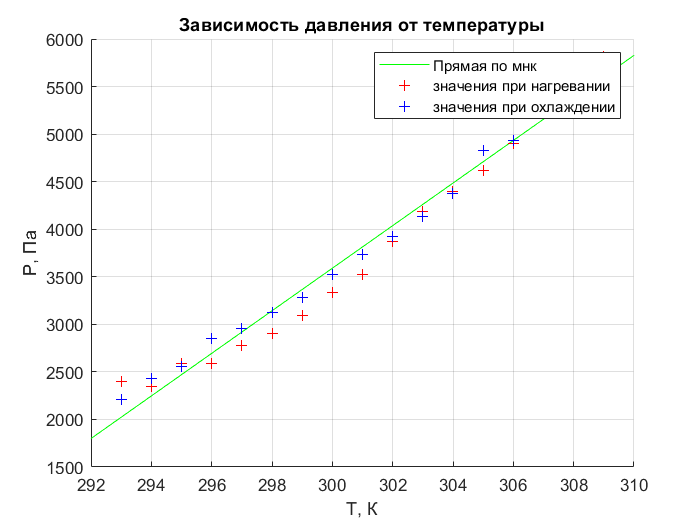
\includegraphics[width=1\linewidth]{plot_2.png}}
\label{plot_1}
\end{figure}
\paragraph{График зависимости $ln\frac{P}{P_0}(T^{-1})$:} 
Аналогично простроим график по всем значениям (нагревание + охлаждение) для зависимости $ln\frac{P}{P_0}(T^{-1})$ (график 2). Здесь $x\Rightarrow(1/T), y\Rightarrow ln(P/P_0) $ Определим константы, необходимые для подсчета коэффициента $b_2$ в этом случае:\\
$\langle 1/T \rangle = 3,323$\\ 
$\langle ln(P/P_0) \rangle = 0,422$\\
$\langle 1/T^2 \rangle = 11,046$\\
$\langle ln(P/P_0)^2 \rangle = 0,265$\\
$\langle 1/T*ln(P/P_0) \rangle = 1,385$\\
Бралось $ N = 33$ точек для аппроксимации. \\
По формуле \ref{mnk} расчитаем коэффициент b:
\[b_2 = \frac{1,385-3,323*0,422}{11,046 - 3,323^2}\approx -5,41 * 10^3 K,\]
\begin{figure}[h]
\center{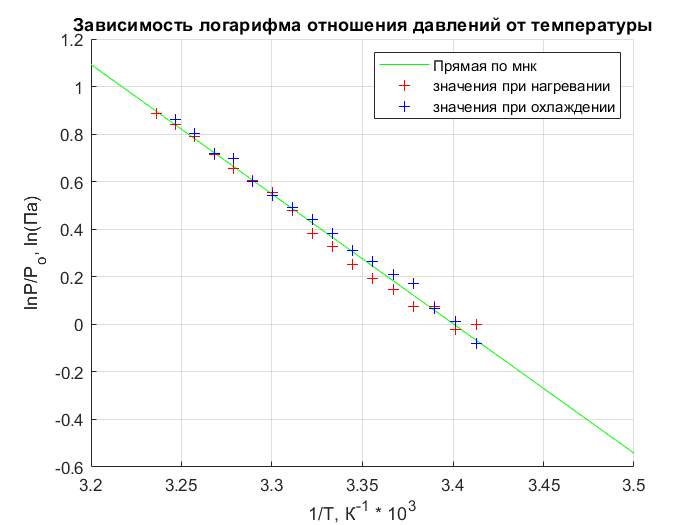
\includegraphics[width=1\linewidth]{plot_1.png}}
\label{plot_2}
\end{figure}
\item
\paragraph{ По формуле (2) вычислим $L$, пользуясь данными 1 и 2 графиков.}
\[L=\frac{ RT^2}{P}\frac{dP}{dT} = b_1\frac{RT^2}{P}\ = 226\frac{8,31*301^2}{3820}\approx 44500\frac{\text{Дж}}{\text{моль}}\]
\[L = - R\frac{d(lnP)}{d(\frac{1}{T})} = - R*b_2 = 8.314 * 5.41 * 10^3 \approx 45200 \frac{\text{Дж}}{\text{моль}}.\]
\paragraph{Найдем погрешности:}
\paragraph{}
Погрешности коэффициентов и $b_i$ находим по формуле:
\begin{equation}
\sigma_b \approx \frac{1}{\sqrt{N}}\sqrt{\frac{\langle y^2 \rangle - \langle y \rangle ^ 2}{\langle x^2 \rangle - \langle x \rangle ^ 2} - B^2} \
\end{equation}
\[\sigma_{b_1} \approx \frac{1}{\sqrt{N}}\sqrt{\frac{\langle P^2 \rangle - \langle P \rangle ^ 2}{\langle T^2 \rangle - \langle T \rangle ^ 2} - b_1^2} = \frac{1}{\sqrt{33}}\sqrt{\frac{ 15845510 -  3820  ^ 2}{ 90625  -  301 ^ 2} - 206^2}\ \approx 6 \]
\[\sigma_{b_2} \approx \frac{1}{\sqrt{33}}\sqrt{\frac{ 0,265 -  0,422  ^ 2}{ 11,046  -  3,323 ^ 2} - (5,31^2 * 10^6)}\ \approx 9 * 10^5 \]
Для L, подсчитанной 1 способом погрешность можно рассчитать по формуле:
\[
\sigma_L = L 
\sqrt{4 \left(\frac{\sigma_T}{T} \right)^2 + 
\left(\frac{\sigma_P}{P} \right)^2 + 
\left(\frac{\sigma_{b_1}}{b_1} \right)^2} = 44500 \sqrt{4 
\left(\frac{0.1}{301}\right)^2 + \left(\frac{13}{3820}\right)^2 + 
\left(\frac{6}{226} \right)^2} \approx 1200 \frac{\text{Дж}}{\text{моль}}.
\]
Во 2 случае погрешность можно рассчитать таким способом:
\[
\sigma_L = L \frac{\sigma_{b_2}}{b_2} = 45200\frac{0,07}{5,31} \approx 600 \frac{\text{Дж}}{\text{моль}}.
\]

Окончательно получим:\\
$L = 44500 \pm 1200 \frac{\text{Дж}}{\text{моль}}$, 
$L = 44200 \pm 600 \frac{\text{Дж}}{\text{моль}}$\\
Погрешность составила:\\
$\epsilon_1 = 3\%$ и $\epsilon_2 = 1,5\%$ \\соответственно
\end{enumerate}
\section{Вывод:}
\begin{enumerate}
\itemsep0em
\item Мы получили значения для молярной теплоемкости, равные $L = 44500 \pm 1200 \frac{\text{Дж}}{\text{моль}}$, 
$L = 44200 \pm 600 \frac{\text{Дж}}{\text{моль}}$ с погрешностями $\epsilon_1 = 3\%$, $\epsilon_2 = 1,5\%$, что является хорошей точностью
\item Видим, что в графике $ln\frac{P}{P_0}(T^{-1})$ присутствует линейная зависимость
\item Получили более точные значение в координатах $ln\frac{P}{P_0}(T^{-1})$
\item Получили разницу между полученным и табличным значениями. Возможно, это связано с недостаточно медленным нагреванием воды.
\end{enumerate}

\end{document}